%% rnaastex.cls is the classfile used for Research Notes. It is derived
%% from aastex61.cls with a few tweaks to allow for the unique format required.
\documentclass{rnaastex}
\usepackage{amsmath, amssymb, bm}
\DeclareMathOperator*{\argmin}{arg\,min}

\newcommand{\todo}[3]{{\color{#2} \emph{#1} TO DO: #3}}
\newcommand{\zetodo}[1]{\todo{ZE}{cyan}{#1}}

%% Define new commands here
\newcommand\latex{La\TeX}

\newcommand{\chicago}{Department of Astronomy and Astrophysics, University of
Chicago, 5640 S. Ellis Ave, Chicago, IL 60637, USA}
\newcommand{\sagan}{Sagan Fellow}

\begin{document}

\title{Point Spread Function Photometry: The Poisson Likelihood and Unbiased Estimations}


%% Note that the corresponding author command and emails has to come
%% before everything else. Also place all the emails in the \email
%% command instead of using multiple \email calls.
\correspondingauthor{Jos\'e Vin\'icius de Miranda Cardoso}
\email{j.demirandacardoso@nasa.gov}

\author{Jos\'e Vin\'icius de Miranda Cardoso}
\affiliation{NASA Ames Research Center, Moffett Blvd, Mountain View, CA 94035, USA}
\affiliation{Bay Area Environmental Research Institute, 625 2nd St Ste. 209, Petaluma, CA 94952}

\author{Geert Barentsen}
\affiliation{NASA Ames Research Center, Moffett Blvd, Mountain View, CA 94035, USA}
\affiliation{Bay Area Environmental Research Institute, 625 2nd St Ste. 209, Petaluma, CA 94952}

\author{Benjamin Montet}
\altaffiliation{\sagan}
\affiliation{\chicago}
%% Note that RNAAS manuscripts DO NOT have abstracts.
%% See the online documentation for the full list of available subject
%% keywords and the rules for their use.
\keywords{point spread function --- statistical estimation --- photometry}

%% Start the main body of the article. If no sections in the
%% research note leave the \section call blank to make the title.
\section{Introduction}

Stellar photometry from charged-couple devices is at the core of astronomical
observations. Often is the case where the astronomical object of interest is isolated
and photometry can be performed by carefully selecting an aperture around the object
and summing up the pixel values, procedure known as aperture photometry. In crowded regions,
conversely, targets are not disjoint and therefore one has to employ point spread
function (PSF) photometry in order to obtain meaningful information about the targets
of interest. Nonetheless, PSF photometry may as well be applied to isolated targets in
order to obtain not only photometry, but also positional information.

\section{PSF Photometry as a Probabilistic Estimation Problem}

Briefly, PSF photometry consists in fitting the parameters of the PSF
(usually integrated flux and center positions), regardless of the nature of the
PSF (discrete or continuous), to a given image. The $\chi^2$ statistic has been traditionally
used to get the best parameters in the maximum likelihood estimation (MLE) sense.

In this letter, we advocate that the $\chi^2$ statistic might not be adequate for PSF
photometry for two main reasons: (I) the assumption of Gaussian distributed data is only
compatible with the nature of pixel data, i.e., positive integer values, in an assymptotic sense;
(II) $\chi^2$ statistic yields a maximum likelihood estimator for the total number of counts
which is biased, and therefore it is only compatible with aperture photometry in an assymptotic sense.
Furthermore, we report that under Poissonian data distributed assumption and for a very
general family of PSF models including, e.g., Gaussian models and discrete models,
the total number of counts obtained using PSF photometry, employing the maximum likelihood
estimator, is equivalent to aperture photometry. As it will be shown, this equivalency is not
valid, e.g., if Gaussian distributed data is assumed.

We begin by stating the underlying statistical assumptions.
Consider an experiment that outputs a stellar image as a collection of $n$ independent \emph{non-identically}
distributed random variables $\bm{Y} \triangleq \{Y_i\}_{i=1}^{n}$ (pixels), each of which has expected value
$\mathbb{E}\left[Y_i\right] = \lambda_i(\bm{\Theta})$, in which $\lambda_i$ is the PSF model evaluated
at the $i$-th pixel, and $\bm{\Theta}$ is a $\Lambda$-valued random vector, where
$\Lambda \subseteq \mathbb{R}^m$ is a compact set that encodes the information about, say, total number
of counts and center positions of the PSF model.

Assuming further that, for a given vector of stellar parameters $\bm{\Theta} = \bm{\theta}$,
$Y_i$ follows a Poisson distribution, then the joint conditional likelihood function of a
stellar image $\bm{Y}$ can be expressed as
\begin{align}
    P(\bm{Y} = \bm{y} | \bm{\Theta} = \bm{\theta}) = \prod_{i=1}^{n} p(y_i | \bm{\theta}) = \prod_{i=1}^{n} \exp{-\lambda_i(\bm{\theta})}\dfrac{\lambda_i^{y_i}(\bm{\theta})}{y_i!} = \exp\left({-\sum_{i=1}^{n}\lambda_i(\bm{\theta})}\right)\prod_{i=1}^{n}\dfrac{\lambda_i^{y_i}(\bm{\theta})}{y_i!}.
\end{align}

Perhaps of more practical interest is the log likelihood function
\begin{equation}
    \log P(\bm{Y} = \bm{y} | \bm{\Theta} = \bm{\theta}) = \sum_{i=1}^{n}\left(- \lambda_i(\bm{\theta}) + y_i\log\lambda_i(\bm{\theta}) - \log y_i !\right).
\end{equation}

Then, the MLE can be stated as follows
\begin{align}
    \bm{\theta}^{*} = \argmin_{\bm{\theta} \in \Lambda} \sum_{i=1}^{n}\left(\lambda_i(\bm{\theta}) - y_i\log\lambda_i(\bm{\theta})\right),
\end{align}
which inevitably requires the solution of the following system of differential equations
\begin{equation}
    \sum_{i=1}^{n}\dfrac{\partial \lambda_i(\bm{\theta})}{\partial \theta_j}\left(1 - \dfrac{y_i}{\lambda_i(\bm{\theta})} \right)\Bigr|_{\substack{\bm{\theta}=\bm{\theta}^{*}}} = 0,~\mathrm{for}~j=1, 2, ..., m.
    \label{eq:partial_eqs}
\end{equation}

As far as the authors are concerned, such a system does not have an analytical solution even for simple PSF models such as Gaussian or Moffat. However, the existence of an MLE is guaranteed since the parameter space is compact and the likelihood function is continuous as a function of $\bm{\theta}$.

Now, assume that the vector of stellar parameters $\bm{\theta}$ takes the following form $\bm{\theta} \triangleq (\alpha, \bm{x})$, where $\alpha$ is the total number of counts and $\bm{x} \triangleq (x_1, x_2)$ is the coordinate of the center of the PSF. Further, assume that the PSF model can be factorized as follows
\begin{equation}
    \lambda_i(\bm{\theta}) = \alpha\cdot\psi_i(\bm{x}),
    \label{eq:psf_model}
\end{equation}
where $\psi_i(\bm{x})$ is the normalized PSF model centered at $\bm{x}$ at the \textit{i}-th pixel, such
that $\sum_{i=1}^{n}\psi_i(\bm{x})=1$.

Therefore,
\begin{equation}
    \dfrac{\partial{\lambda_i(\bm{\theta})}}{\partial \alpha} = \psi_i(\bm{x}).
    \label{eq:partial_flux}
\end{equation}

Substituting (\ref{eq:psf_model}) and (\ref{eq:partial_flux}) into (\ref{eq:partial_eqs}), it follows that
\begin{align}
    \sum_{i=1}^{n} \psi_i(\bm{x}^{*})\left(1 - \dfrac{y_i}{\alpha^{*}\cdot\psi_i(\bm{x}^{*})} \right) &= \sum_{i=1}^{n} \left(\psi_i(\bm{x}^{*}) -  \dfrac{y_i}{\alpha^{*}}\right) = 0 \\
    & \Leftrightarrow \nonumber\\
    \alpha^{*} &= \sum_{i=1}^{n} y_i,
    \label{eq:tada}
\end{align}
which proves our proposition. Note that this result does not require any specific structural form of $\lambda_i$ other than it increases linearly with the total number of counts $\alpha$ for a given fixed position $\bm{x}$.

Furthermore, the MLE for the total number of counts has the following nice properties: (\textrm{I}) it is an unbiased estimator and (\textrm{II}) its variance has a closed-form. The first property may be verified by taking the expectation value of (\ref{eq:tada}), which follows that
\begin{equation}
    \mathbb{E}\left[\alpha^{*}\right] = \sum_{i=1}^{n}\mathbb{E}[Y_i] = \sum_{i=1}^{n} \lambda_i(\bm{\theta}) = \sum_{i=1}^{n} \alpha\cdot\psi_i(\bm{x}) = \alpha.
\end{equation}
To verify the second property, note that $\alpha^{*}$ is the sum of independent Poisson random variables, therefore, $var\left[\alpha^{*}\right] = \mathbb{E}\left[\alpha^{*}\right] = \alpha$.

Note that, under the widely adopted assumption that the data is Gaussian distributed (corresponding to a $\chi^2$ likelihood function), the solution for $\alpha^{*}$ would be
\begin{equation}
    \alpha^{*} = \dfrac{\sum_{i=1}^{n}y_i \psi_i(\bm{x}^{*})}{\sum_{i=1}^{n}\psi^2_i(\bm{x}^{*})},
\end{equation}
for which, properties (I) and (II) do not hold in an non-asymptotic sense.

As a practical exercise, we apply PSF photometry on EPIC 2307199
\begin{figure}
    \centering
    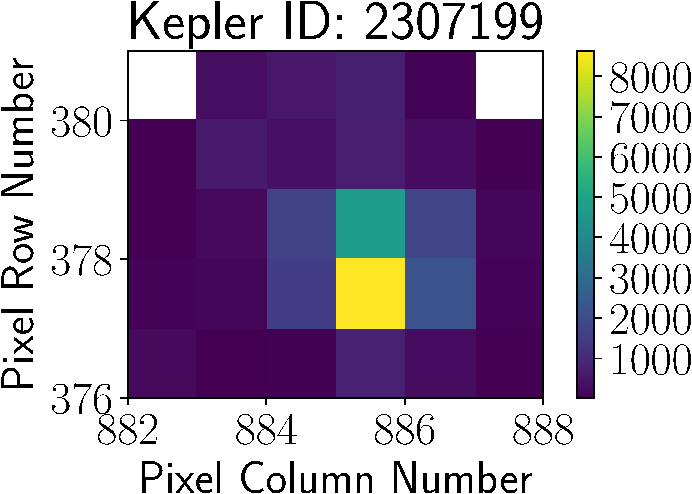
\includegraphics[scale=.37]{tpf.pdf}
    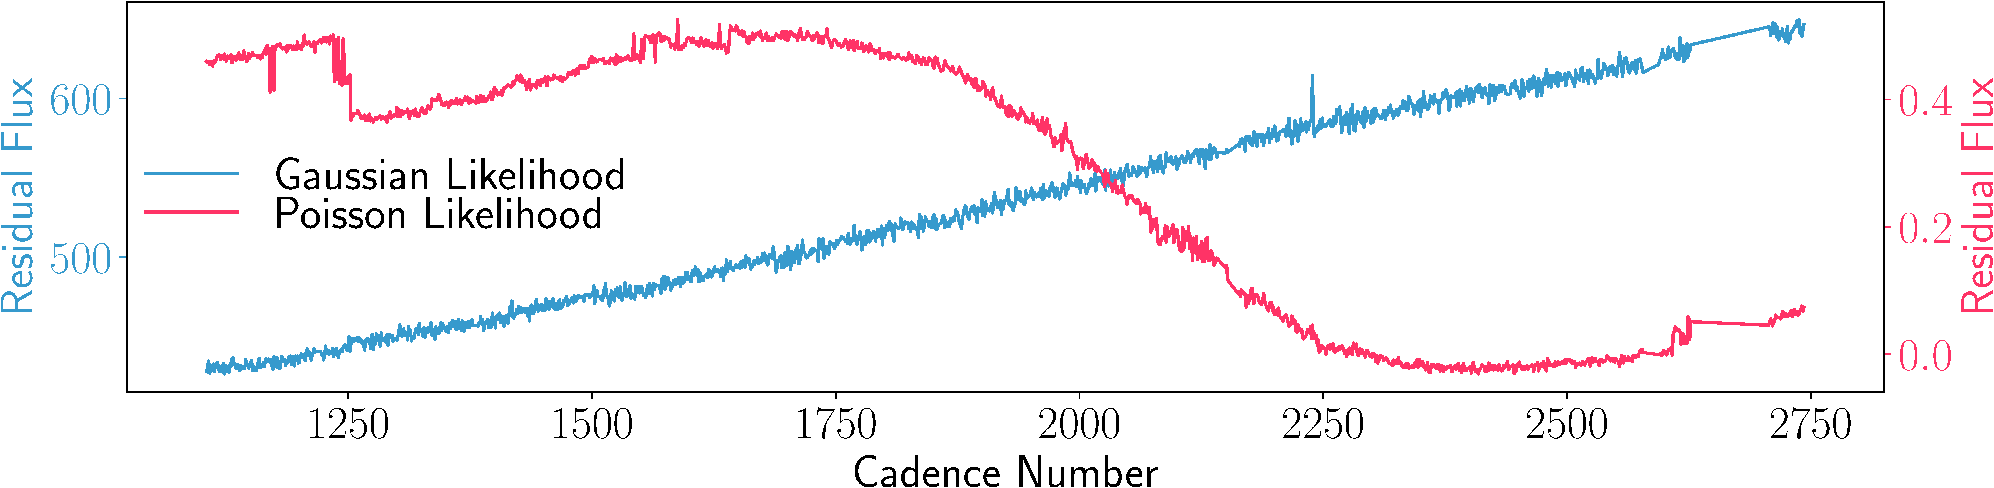
\includegraphics[scale=.37]{residuals.pdf}
    \caption{(left): cadence \#2000 of EPIC 230719 from NASA's Kepler Mission. (right): residuals per cadence of PSF photometry using Poisson Likelihood (red) and Gaussian Likelihood (blue).}
\end{figure}

The code is available at:

\acknowledgments We would like to thank

\begin{thebibliography}{}

\end{thebibliography}

\end{document}

